
\chapter{Introduction}
\label{chap:Introduction} 

\lettrine{T}{his} project investigates the newly discovered family of 
pentatricopeptide repeat (PPR) proteins, which are vital to plant biology and 
could become an exciting new tool in the field of synthetic biology.
The project spans the space between engineering and the life-sciences and this
section provides an introduction to the relevant fields and the motivation
behind the project.

\section{Molecular Biology}
\label{sec:MolecularBiology}

Molecular biology is the study of the molecular basis of biology.
It is mostly concerned with the understanding of the systems and processes
that occur within a living cell.
Naturally, the field overlaps considerably with other areas, 
such as genetics (the study of genes and heredity) and biochemistry (the study
of the chemical processes of life).

While the field itself is rather broad, much of it is underpinned by what is
referred to as the central dogma of molecular biology -- 
DNA makes RNA makes proteins.
This central dogma describes the flow of information within a cell and the
mechanisms which regulate this flow.
Many of these processes are highly complicated and remain poorly
understood, but much progress has been made since the discovery of DNA in the
1950s to understand these mechanisms.
Figure~\ref{fig:processes} shows the most important of these and how
they convert between the three most important classes of molecules in the cell.

\begin{figure}
  \centering
  \begin{tikzpicture}[node distance=5cm, auto,
      general/.style={->, >=triangle 60},
      special/.style={->, dashed, >=triangle 60}]
    \node (D) {DNA};
    \node (R) [right of=D] {RNA};
    \node (P) [right of=R] {Protein};
    \draw[general, bend left] (D) to node {\small \textit{transcription}} (R);
    \draw[general, bend left] (R) to node {\small \textit{translation}} (P);
    \draw[general] (D) to [out=110,in=70,looseness=8] 
          node[anchor=south east] {\small\textit{DNA replication}} (D);

    \draw[special, bend left] 
      (R) to node {\small \textit{reverse transcription}} (D);
    \draw[special] (R) to [out=335,in=295,looseness=8] 
                node {\small\textit{RNA replication}} (R);
  \end{tikzpicture}
  \caption{The main processes in molecular biology. The three most common are
    shown using solid lines while two important but less common processes are
    shown in dotted lines.
    \label{fig:processes}}
\end{figure}

Molecules of DNA are the cell's long term storage mechanism -- recent research
estimates the half-life of DNA to be 521 years \citep{DNAhalflife}.
DNA molecules are long sequences of simple molecules called nucleotides, the
sequence of  which encodes all the genetic information of the cell.
Each nucleotide contains a nucleobase which is either Adenine, Guanine,
Thymine or Cytosine (A, C, G or T) and it is the sequence of bases 
which determines the information content of the molecule.
The nucleotides are linked together in a strand which is only read in one 
direction, known as the 5' to 3' direction.

These strands do not normally exist independently, but instead form hydrogen
bonds with each nucleobase in a complementary strand, forming double stranded
DNA.
The sequence of the complementary strand is determined by the hydrogen bonds
formed between bases -- A binds with T, G binds with C.
The strands bind such that they are read in opposite directions -- the 5' to 3' 
direction on the reverse strand is in the reverse direction to that of the 
forward strand -- hence converting a sequence from the
forward to reverse strand is referred to as a \emph{reverse complement}.

The two strands are coiled around each other into DNA's characteristic 
double-helix structure.

\begin{figure}
  \centering
  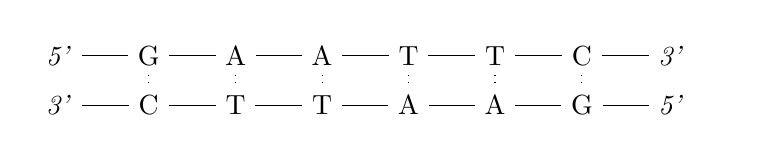
\begin{tikzpicture}[auto, node distance=2cm,>=latex]
    % We start by placing the blocks
    \matrix[row sep=0.15cm, column sep=0.6cm] {
      \node[name=a5p] {\emph{5'}}; &
      \node[name=a1] {G}; &
      \node[name=a2] {A}; &
      \node[name=a3] {A}; &
      \node[name=a4] {T}; &
      \node[name=a5] {T}; &
      \node[name=a6] {C}; &
      \node[name=a3p] {\emph{3'}}; &
    \\
      \node[name=b3p] {\emph{3'}}; &
      \node[name=b1] {C}; &
      \node[name=b2] {T}; &
      \node[name=b3] {T}; &
      \node[name=b4] {A}; &
      \node[name=b5] {A}; &
      \node[name=b6] {G}; &
      \node[name=b5p] {\emph{5'}}; &
    \\};

    \draw (a5p) to (a1);
    \draw (a1)  to (a2);
    \draw (a2)  to (a3);
    \draw (a3)  to (a4);
    \draw (a4)  to (a5);
    \draw (a5)  to (a6);
    \draw (a6)  to (a3p);

    \draw (b3p) to (b1);
    \draw (b1)  to (b2);
    \draw (b2)  to (b3);
    \draw (b3)  to (b4);
    \draw (b4)  to (b5);
    \draw (b5)  to (b6);
    \draw (b6)  to (b5p);

    \draw[dotted] (a1) to (b1);
    \draw[dotted] (a2) to (b2);
    \draw[dotted] (a3) to (b3);
    \draw[dotted] (a4) to (b4);
    \draw[dotted] (a5) to (b5);
    \draw[dotted] (a6) to (b6);
  \end{tikzpicture}
  \caption{
    An example of a DNA fragment. 
    Covalent bonding along the strands is shown with solid lines and hydrogen 
    bonding between the two strands is shown using dotted lines.
    In this case the forward and reverse strand happen to be palindromic, 
    although this is by no means necessary.
    Note that the decision as to which strand is considered the forward and
    which is the reverse is arbitrary -- in fact other naming schemes (such as
    Watson/Crick) also exist.
  }
  \label{fig:dna_pairing}
\end{figure}


The data stored in DNA is read by a molecule called RNA polymerase which 
produces a single stranded RNA copy of a section of the DNA in a process called
\textit{transcription}.
RNA is similar to DNA, but is short-lived (lasting minutes to hours) and so the
RNA copy is referred to as a messenger-RNA (mRNA) molecule.
This message is then read by a ribosome, a molecule which translates the mRNA 
into a protein in a process referred to as \textit{translation}.
Proteins are linear chains of amino acids linked by flexible joints which fold 
into a very specific shape and perform many important functions within the 
cell.
The region of DNA which codes for a particular protein is called a 
\textit{gene}.

The processes of transcription and translation through which genes are 
expressed (produce proteins) are typically very tightly
controlled by the cell, as this is the main way of influencing the levels of
various proteins within the cell and thus the cell's overall activity.

\subsection{Transcription}
\label{sec:transcription}

Both DNA and RNA have an alphabet of four symbols and so during transcription
DNA's alphabet, $\{A,C,G,T\}$, is mapped directly to that
of RNA, $\{A,C,G,U\}$, where thymine is replaced with uracil.
Transcription is clearly bijective, and indeed a less common process called
reverse-transcription performs the inverse mapping from RNA to DNA.

Transcription does not act on an entire DNA strand at once but instead
transcribes a subsequence of the DNA called a transcription unit, which
contains one or many genes.
These units are marked by promoters which are regions of DNA upstream
of the transcription unit that initiate transcription by causing RNA polymerase
to bind.
Modulating promoter activity in response to the concentration of another 
molecule is a common control motif.
Transcription units are terminated by terminator regions, which cause the RNA 
polymerase to cease transcription and release the mRNA.

Transcripts often include non-coding regions at either end called the 5' and 3'
untraslated regions (UTR) respectively.
They also contain other non-coding regions called \textit{introns}
which often found within gene sequences and are removed from the message in a 
process called RNA splicing before translation.
Introns do not contain any useful sequence and tend to complicate matters 
significantly as efforts to predict their location accurately and reliably 
have thus far failed -- they are best detected using reverse transcription.

\subsection{Translation}
\label{sec:translation}

Translation is the process by which an RNA message is converted into a protein.
In higher cells (eukaryotes), mRNA undergoes further processing and is exported
from the nucleus before translation while lower organisms (prokaryotes)
translation begins immediately, possibly concurrently with
transcription.

Proteins are a sequence of amino acids, where each acid comes from an alphabet
of 20 amino acids.
Each acid is coded for by 3 bases of RNA, which are referred to collectively 
as a codon.
Since there are 64 possible codons and only 20 amino acids, the code is
overcomplete -- several different codons map to the same amino acid -- and
thus a definitive reverse mapping from protein to DNA sequence is impossible.
As well as coding for amino acids, special codons mark the start and end of a
protein.
A start codon (AUG) marks the beginning of a protein and one of the three stop 
codons (UAG, UAA and UGA) terminate the translation of the protein.

In translation, molecules called ribosomes bind to the mRNA, reading the
sequence 3 bases (one codon) at a time and constructing the appropriate protein
until a stop codon is found, when the ribosome detaches and releases the
protein.
The point where the ribosome binds is called a ribosome binding sequence (RBS),
a common class of which is the Shine-Dalgarno sequence, which is found a few 
bases upstream of the start codon.

Because of the 3:1 nature of translation, proteins are sensitive to frame
shifts -- where translation is shifted by one or two bases, the resulting amino
acid sequence is effectively unrelated to the encoded one.
This can be the case if an unexpected intron is present as introns need not be 
multiples of three codons long.

mRNA is more fragile than DNA but is also targeted by exonucleases, a class of
enzyme which degrade RNA molecules, preventing the production of more protein.
Similar processes exist which degrade proteins over time, recycling their amino
acids to form new proteins.
These degradation processes mean that a gene must continue to be 
\emph{expressed} (transcribed and translated) at a constant rate for the 
concentration of its protein to remain constant.

\subsection{Controlling Expression}
\label{sec:mbio_control}

\begin{figure}
  \begin{center}
    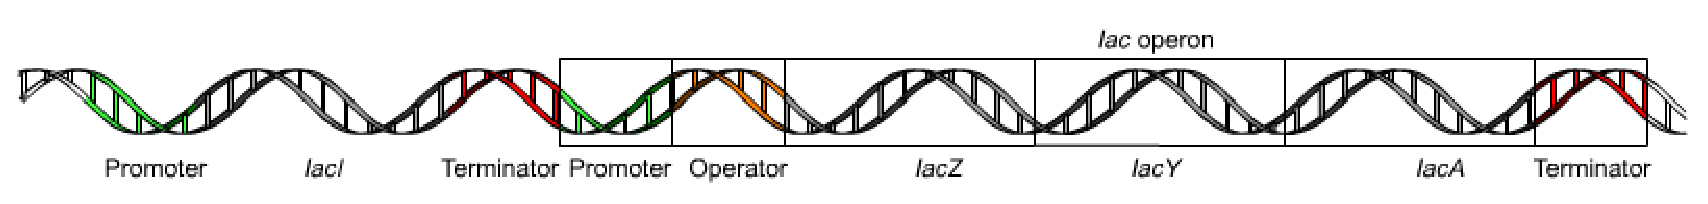
\includegraphics[width=\textwidth]{Lac_operon1}
  \end{center}
  \caption[LoF entry]{Annotated diagram of the lac operon.
    It contains two transcription units and a total of four genes.
    The first (leftmost) unit contains the \textit{lacI} gene and is expressed 
    constitutively (continuously).
    The protein which is produced is called the lac repressor, and in the
    absence of lactose it binds tightly to the operator region, preventing
    transcription of the second transcriptional unit.
    However, when lactose is present outside the cell, a small amount will
    diffuse across the cell wall and into the cell, where it binds with the lac
    repressor, preventing it from binding to the operator and allowing
    transcription of the second unit.
    
    Of the three genes that are then expressed, two are directly relevant.
    \textit{lacY} encodes a membrane protein which actively pumps more lactose
    into the cell, causing positive feedback, and \textit{lacZ} which produces
    an enzyme which breaks down lactose into glucose and galactose which can be
    metabolised more easily.
    
    Glucose in the cell interacts with the membrane protein, reducing the rate
    at which it imports lactose and introducing a second control loop.
    As the concentration of glucose increases, less lactose is pumped into the
    cell and so the lac operon becomes less active, reducing transcription of
    the second unit.
  }
  \label{fig:lac_operon}
\end{figure}



\begin{figure}
  \centering
  \begin{tikzpicture}[auto, node distance=2cm,>=latex]
    % We start by placing the blocks
    \matrix[ampersand replacement=\&, row sep=0.15cm, column sep=0.6cm] {
      \&
      \&
      \&
      \node [block] (break) {Lactose Breakdown}; \&
      \&
    \\
      \node [input, name=glu] {}; \&
      \node [sum] (s3) {}; \&
      \node [block] (gsense) {Sensor}; \&
      \&
      \&
    \\
      \&
      \&
      \&
      \node [sum] (s2) {}; \&
      \node [branch] (br) {}; \&
      \node [output] (out) {}; 
    \\
      \node [input, name=lac] {}; \&
      \node [sum] (s1) {}; \&
      \node [block] (lsense) {Sensor}; \&
      \&
      \&
      {}; 
    \\
      \&
      \&
      \&
      \node [block] (import) {Lactose Importing}; \&
      \&
    \\};

    \node [label, right of=out, node distance=1cm] {operon\\activity};
    

    % Once the nodes are placed, connecting them is
    % easy. 
    \draw [draw,->] (glu) -- node[pos=0.01] {$[glu]$} (s3);
    \draw [->] (s3) -- (gsense);
    \draw [->] (lac) -- node[pos=0.01,swap] {$[lac]$} (s1);
    \draw [->] (s1) -- (lsense);
    \draw [->] (lsense) -| node[pos=0.95]       {$+$} (s2);
    \draw [->] (gsense) -| node[pos=0.95, swap] {$-$} (s2);
    \draw [- ] (s2) -- (br);
    \draw [->] (br) -- (out);
    \draw [->] (br) |- (import);
    \draw [->] (br) |- (break);
    \draw [->] (import) -| node[pos=0.95, swap] {$+$} (s1);
    \draw [->] (break)  -| node[pos=0.95] {$+$} (s3);

  \end{tikzpicture}
  \caption{Simplified block diagram of the lac operon, showing only the most
    important interconnections. 
    In the presence of lactose, transcription is turned on and more
    extracellular lactose is pumped into the cell, causing a positive feedback
    loop.
    Simultaneously, lactose is broken down into glucose (and galactose) which
    inhibits transcription, causing a negative feedback loop.
  }
  \label{fig:lac_block}
\end{figure}

Control of protein production is typically achieved using several layers of
control at different stages.
For example, the lac operon controls the production of enzymes which allows the
cell to metabolise lactose, a carbon source.
The cell would prefer to directly metabolise glucose if it is available as
lactose is harder to process, and so the cell can save energy by only turning
on its lactose processing machinery when only lactose is available.
This is achieved by the lac operon as described in figure~\ref{fig:lac_operon} 
and shown schematically in figure~\ref{fig:lac_block}.

Although the lac operon was one of the first such control structures to be
discovered (and remains among the best understood), many other ingenious ways
of tightly controlling protein production have been discovered, some of which
act on transcription, some on translation and others on a combination of the
two.

\section{Synthetic Biology}
\label{sec:synbio}

Synthetic biology is a relatively new
engineering discipline with the goal of applying proven engineering techniques
such as standardisation, characterisation and encapsulation to biology.
Synthetic Biology aims to use these design principles to combine existing 
phenomena to build new, artificial forms of life.
The field is often confused with its spiritual predecessor, genetic 
engineering, which although similar in some respects does not design new
organisms, but tinkers with existing ones without trying to understand the
underlying principals.

Synthetic biology can be thought of as programming, but with DNA instead of 
machine code.
An example project which nicely captures this idea is Tabor's bacterial edge
detector \citep{edgeDetector}.
Bacteria were programmed to produce a colourless chemical messenger in the 
absence of light and to produce a dark pigment in the presence of both light 
and the chemical messenger.
When a film of these bacteria is exposed to a pattern of light and dark, the
messenger is produced in the dark regions and diffuses into the light, where it
stimulates the production of the pigment, 
leading to an edge detection effect.

While this and other such simple demonstrations show some of the potential 
of synthetic biology, they lack immediate application and are of somewhat 
limited scope.
A major problem in expanding this work is the lack of targeted reporter
molecules.
In the edge detector example, two molecular signals are produced when light is 
not present -- AHL, a cell-to-cell signalling molecule and cI, a
transcriptional repressor molecule.
Both AHL and cI are known to affect the promoter $P_{lux-\lambda}$; while AHL 
stimulates expression, cI strongly represses it.
With expression of the dark pigment being driven by $P_{lux-\lambda}$, 
both light and AHL are required to cause the pigment to be produced.

The effect of the molecules AHL and cI on $P_{lux-\lambda}$ is one of a small
but growing number of well understood control motifs.
Since reusing the same promoter/signal combination in the same cell is 
impossible due to cross-talk, there are simply not enough signalling modalities 
or characterised promoters available to perform more complex logic within the 
cell.
Indeed, it is often the case that signalling molecules have multiple functions
within the cell such that changing the concentration of one molecule to suit
our goals may cause a seemingly unrelated area of the cell's metabolism to
malfunction with undesirable consequences.

A quite separate and more applicable project was the effort to produce 
artemisinin (the most effective known anti-malarial) in a cheaper and more 
scalable way.
Malaria is a treatable disease which caused roughly 2,000 deaths 
\emph{per day} in 2010, mainly because it mostly affects the developing world 
where access to anti-malarials is poor \citep{malaria}.
Artemisinin is found naturally in sweet wormwood, but it is slow and expensive
to extract directly from the plant and chemical synthesis is also an expensive
and laborious process.
Synthetic biologists were able to extract the metabolic pathway responsible for
the biosynthesis of artemisinic acid (a natural precursor) and insert it into 
yeast \citep{yeast}.
Artemisinin produced in this manner has yet to be approved for sale, but it is
hoped that it should be available at some point during 2013, at a considerably
lower price than any other known method of production.

The major limiting factor in this project was yield.
In order to produce a useful amount of the drug, the metabolic pathway 
involved had to be up-regulated -- i.e. more metabolic flux directed though it.
This led to a difficult balance -- too little and very little
artemisinic acid would be produced, too high and too much of the cell's
energy would be used, causing the cells to grow slowly if at all.
As well as this, growing yeast on an industrial scale is relatively expensive.
It is desirable therefore search for host platforms which are better suited to
biosynthesis than yeast, in order to maximise the yield to cost ratio.

\section{The Chloroplast}
\label{sec:intro_chloroplast}

Chloroplasts are a major centre for biosynthesis in plants as they perform
photosynthesis to provide energy for the plant.
The result of an ancient symbiosis, up to 1000 of these primitive cells can be 
found within each plant cell, where they make an excellent target for synthetic
biology.
Their primitive nature makes them similar to previous hosts, 
but with access to the more sophisticated plant cell machinery and 
superb potential for biosynthesis.
For example, the native enzyme RuBisCO is so abundant in the chloroplasts that 
it can represent up to 50\% of overall soluble leaf protein.

Chloroplasts contain limited genetic information and expression machinery 
separate from that of the plant cell, which produces the molecules required 
for expression and several proteins vital to the photosystem.
However, many proteins found in the chloroplast are in fact produced by the
nucleus and then imported into the chloroplast.

The style of operon-based control common in prokaryotic cells does not appear 
to be used in the chloroplast -- instead most genes are 
transcribed constitutively \citep{Sugita1996}, leading to constant mRNA levels.
It is also known that the mRNA transcripts in chloroplasts often do not 
contain a ribosome binding site (such as a Shine-Dalgarno sequence) at all or 
that such a sequence is not in the correct 
location \citep{Sugiura1998,Zerges2000}.

This does not reflect the clear variation in protein levels found in the 
chloroplast, whose activity varies considerably during the chloroplast's 
circadian cycle -- energy is stored during the day and consumed at night.
Since mRNA levels are constant, this control must occur at a 
post-transcriptional level, and there is evidence to suggest that the nucleus
is involved in controlling the cycle \citep{Matsuo2006}.

Chloroplast mRNAs also undergo significant post-transcriptional processing such
as C-U editing (where a genome-encoded C is converted to a U) and less 
commonly, U-C editing \citep{Castandet2011}.
The underlying purpose of this RNA editing remains an open question. 
One theory is that it corrects for unfavourable mutations which have
accumulated in the chloroplast genome and that removing these changes 
artificially would increase the efficiency of the plant \citep{Fujii2011}.
However, it is also possible that editing is a vital method allowing to nucleus
to tightly control expression in the chloroplast and that removing the 
mutations would result in plants which were unable to control their 
chloroplasts.

Understanding regulation in chloroplasts is a vital step before they can be
effectively used for synthetic biology.
For example, attempting to synthesise useful chemicals at the wrong point in 
the circadian cycle would likely result in very poor growth and so we must be
able to tap into the natural regulation system already present in the system.

\section{Nucleotide Binding Proteins}
\label{sec:intro_binding}

Accurately predicting the structure of a protein from its amino acid sequence 
is very difficult and in most cases impossible.
The main difficulty is that the joints between amino acids in a protein are
very flexible, giving amino acids a very high number of degrees of freedom,
which often thwarts attempts to find the structure with minimum free energy.
Even when this can be found, protein folding is often a complex process
involving several interactions with other chaperone proteins which guide
protein folding, meaning that the global minimum energy solution may not 
represent the actual shape of the protein.

As a result, modelling interactions between proteins and nucleotides such as
DNA and RNA is impossible in the general case and these interactions are
instead found and characterised using empirical techniques.

One of the first such interactions to be discovered were zinc fingers, a
protein motif whose folding structure is stabilised by the incorporation of a
zinc ion into the structure.
Zinc fingers are common in many organisms and recognise and bind to a specific 
triplet of nucleotides, and have been reverse-engineered such that they can now
be designed to bind to effectively arbitrary sequences \citep{Gaj2013}.

However, zinc fingers have limited modularity as each motif binds to three
bases with varying specificity, meaning that there are often other sequences to
which the protein will bind which can be hard to predict.
Transcription activator-like effectors (TALEs) are modular repeat regions in
which each repeat recognises a single DNA base via a simple code dependent on
two hyper-variable amino acids within the repeat motif.
The superior modularity of TALEs make them inherently easier to design than 
zinc fingers and have been used for
numerous novel applications, such as designing new transcription activators
which work on arbitrary sequences or manipulating the genome to allow for novel
studies of protein function \citep{Sun2013}.

These two classes of proteins have opened up new and exciting methods for basic
research, gene therapy and synthetic biology.

\section{The PPR Family}
\label{sec:review_PPR}
\subsection{Discovery and Classification of the PPR Family}

\begin{figure}
  \begin{center}
    \begin{tikzpicture}
      \def\h{5mm}
      \def\n{10}
      \tikzstyle{signal}=[draw, rectangle, minimum height=\h, minimum
        width=2cm, anchor=west]
      \tikzstyle{motif}=[draw, rectangle, fill=orange, 
        minimum height=\h, minimum width=8mm, anchor=west]
      \tikzstyle{tail}=[draw, dashed, rectangle, fill=blue!20,
        minimum height=\h, minimum width=3cm, anchor=west]

      \tikzstyle{brace}=[
        very thick,
        decoration={
          brace,
          mirror,
          raise=5mm
        },
        decorate]

      \node[signal, name=signal] at (-2,0) {};
      \foreach \y in {1,...,\n}{
        \node[motif] at ({0.8 * (\y-1)},0) {};
      }
      \node[tail, name=tail] at ({0.8 * \n},0) {};

      \draw [brace] (-2,0) -- (-0.1,0)
        node [key, pos=0.5,anchor=north,yshift=-7mm] {A}; 
      \draw [brace] (0.1,0) -- ({0.8*\n - 0.1},0) 
        node [key, pos=0.5,anchor=north,yshift=-7mm] {B}; 
      \draw [brace] ({0.8*\n+0.1},0) -- (tail.east) 
        node [key, pos=0.5,anchor=north,yshift=-7mm] {C}; 
    \end{tikzpicture}
  \end{center}
  \caption[LoF entry]{
    The three regions within a PPR protein.
    (\textbf{A}) The signal peptide acts as a header, essentially encoding the
    address of the target location of the PPR within the cell
    (\textbf{B}) The repeat regions contain 2-30 PPR motifs which specify the binding
    preferences of the protein
    (\textbf{C}) The tail region is optional contains either E, E and E+ or 
    E, E+ and DYW motifs.
  }
  \label{fig:ppr_anatomy}
\end{figure}

The PPR family is a group of proteins commonly found in plants and are known
to bind specific RNA sequences and display many similarities with TALEs.
They contain tandem degenerate repeating motifs which are referred to as PPR 
motifs and share many similarities with the tetratricopeptide repeat (TPR) 
motif which are known to aid protein-protein binding \citep{Small2000}.

PPRs are found exclusively in the nuclear genome, and are commonly targeted to
organelles such as the chloroplast or mitochondria, where they are known to
affect translation in numerous ways.

The typical PPR protein contains three regions, shown in figure
\ref{fig:ppr_anatomy}.
The first is a signal peptide which targets the protein to a particular 
organelle.
This mechanism is common to many proteins which are sent to particular
locations within the cell (such as the chloroplast of mitochondria) and not a
particularity of the PPR family. 

The second region is the repeating PPR motif array which contains between 2 and
30 PPR motifs.
The motifs are degenerate -- although they contain many similarities, they are
not identical and in fact have quite considerable differences in some cases.
The standard PPR motif is the P motif which is 35 amino acids long, 
but long (L) and short (S) variants are common in some proteins.
The PPR motifs cause the protein to bind tightly to a specific mRNA sequence,
and it is believed that pairs of contiguous motifs confer the particular
protein's binding preference \citep{Kobayashi2012}.

The third region is a tail sequence which is only present in some PPRs.
The tail regions are known to contain a number of other motifs whose exact
function is unknown.
Three main classes of tail sequence have been identified, 
the E subgroup which contains
only `E' motifs, the E+ subgroup which contains `E' and `E+' motifs and the DYW
subgroup which contains `E', `E+' motifs and is terminated by a `DYW' motif
\citep{Lurin2004}.
The precise function of the tail remains unknown, but evidence suggests that it
is related to the known RNA editing functions of some PPRs \citep{Yagi2013a}.

\subsection{Known interactions with mRNA}

PPRs can regulate gene expression and are involved in a variety of
post-transcriptional RNA processing steps such as RNA editing, splicing and
stability \citep{Schmitz-Linneweber2008,Nakamura2012}.

\subsubsection{RNA editing}

\begin{figure}
  \begin{center}
    \begin{tikzpicture}
      \node[anchor=south west,inner sep=0] (image) at (0,0)
      {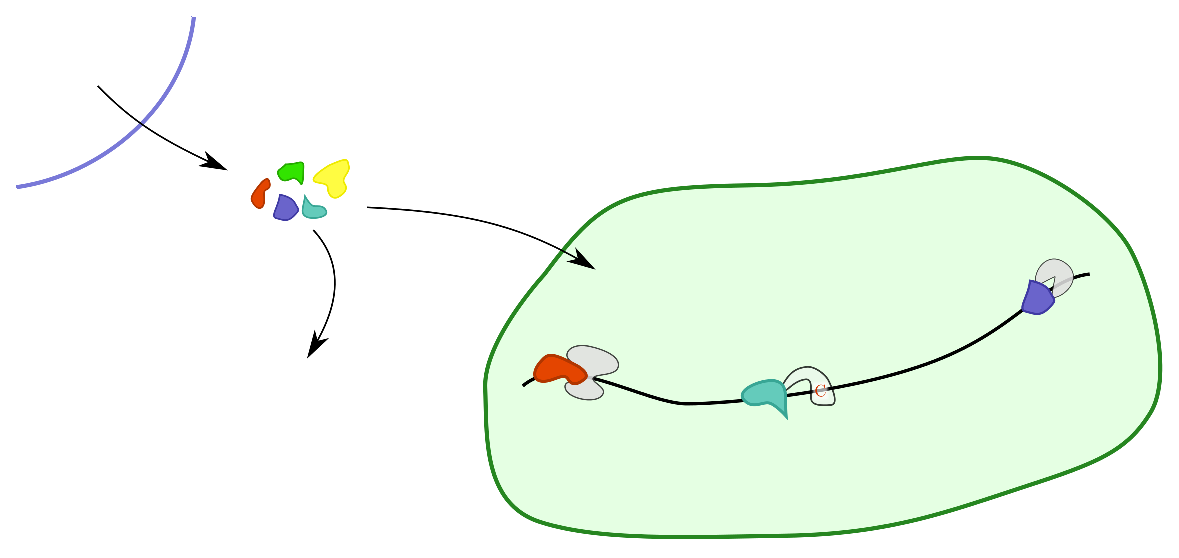
\includegraphics[width=0.9\textwidth]{PPR_activity}};
      \begin{scope}[x={(image.south east)},y={(image.north west)}]
        \node[align=center] at (0.65,0.6) {Chloroplast};
        \node[align=center] at (0.05,0.92) {Nucleus};
        \node[align=center] at (0.2,0.25) {Mitochondria};
        \node[align=center] at (0.25,0.8) {PPR\\Proteins};

        \node[key] at (0.48,0.2) {A};
        \node[key] at (0.67,0.18) {B};
        \node[key] at (0.92,0.38) {C};
      \end{scope}
    \end{tikzpicture}
  \end{center}
  \caption{Summary of PPR activity once in the chloroplast. Similar processes
    are known to occur in the mitochondria.
    (\textbf{A}) Increased translation -- PPRs can promote ribosome recruitment
      and increase the translation rate of the transcript
    (\textbf{B}) RNA editing -- PPRs edit the RNA transcript, as well as
      playing a vital role in the removal of introns
    (\textbf{C}) RNA stability -- PPRs can increase the stability
      of the transcript by protecting against degradation by endonucleases, or 
      decrease the stability, possibly by recruiting endonucleases.
  }
  \label{fig:PPR_activity}
\end{figure}


Several PPR proteins with tail motifs have been associated with RNA editing and
in these cases the PPR binding site has been located a short distance from the
edit site \citep{Okuda2007,Yagi2013a}.
A particular protein can be responsible for several edits by having multiple
binding sites within the chloroplast genome \citep{Okuda2012}, allowing a single
protein to edit multiple genes.

C-U RNA editing has vital consequences for protein translation.
Proteins begin with a start codon (AUG), which marks the position where
translation should start.
If instead the genome codes an ACG codon then the protein will not be expressed
unless a C-U edit event occurs.
Conversely, if a CAA codon is present in the gene, then an RNA
editing event could convert this to UAA -- a stop codon, causing translation to
be terminated.

\subsubsection{Increasing Translation}

It has been shown that PPR binding to the 5' and 3' UTRs can stabilise mRNA
transcripts and reduce degradation by
ribonucleases \citep{Pfalz2009,Prikryl2011}.
This increases protein yield as more mRNA will be present at any time,
increasing the rate at which protein is created.
In addition to stabilisation, PPR binding can facilitate ribosome recruitment
and can thus be responsible for the initiation of translation.

\subsubsection{Decreasing Translation}

PPRs have been shown to be responsible for restoring fertility to plants
affected by Cytoplasmic Male Sterility (CMS) \citep{Bentolila2002}, which is of
commercial importance in breeding.
PPRs prevent sterility by preventing the production of specific proteins which
cause the condition \citep{Kazama2008}.
While the specific interaction preventing translation is unknown, it is thought
to be due to cleavage of the mRNA transcript or degradation \citep{Wang2006}.
It is also possible that the PPR out competes the ribosome when binding to the
ribosome binding site.

\subsubsection{Binding Rules}

The mechanism behind PPR-RNA interactions remains unknown, and it is not yet
possible to accurately predict PPR binding domains from the amino acid sequence
of the protein.
One problem is that the exact structure of the tandem PPR motifs is not known,
although other proteins which also contain PPR motifs appear to show a helical
structure \citep{Ringel2011,Howard2012}, suggesting that PPR binding might be
similar to that of TALE and PUF repeats \citep{Rubinson2012}.

As of writing, two major theories on the PPR binding rules exist, one due to
Barkan \citep{Barkan2012} and another due to Yagi \citep{Yagi2013}.
Both are based on statistical inference on the small number of characterised
PPR-RNA interactions and are discussed in more length in section
\ref{sec:ppr_binding_prediction}.

\section{Hidden Markov Models}
\label{sec:HMMs} 

\begin{figure}
  \begin{center}
    \begin{tikzpicture}[node distance=2cm, auto, >=triangle 45]
      \node [match, name=begin] {Begin};
      \node [match, name=m1, right of=begin] {};
      \node [match, name=m2, right of=m1] {$M_j$};
      \node [match, name=m3, right of=m2] {};
      \node [match, name=end, right of=m3] {End};

      \node [insert, name=i0, above of=begin] {};
      \node [insert, name=i1, above of=m1] {};
      \node [insert, name=i2, above of=m2] {$I_j$};
      \node [insert, name=i3, above of=m3] {};

      \node [delete, name=d1, above of=i1] {};
      \node [delete, name=d2, above of=i2] {$D_j$};
      \node [delete, name=d3, above of=i3] {};

      %matches
      \draw [->] (begin) to (m1);
      \draw [->] (begin) to (i0);
      \draw [->] (begin) to (d1);
      \draw [->] (m1) to (m2);
      \draw [->] (m1) to (i1);
      \draw [->] (m1) to (d2);
      \draw [->] (m2) to (m3);
      \draw [->] (m2) to (i2);
      \draw [->] (m2) to (d3);
      \draw [->] (m3) to (end);
      \draw [->] (m3) to (i3);

      %inserts
      \draw [->] (i0) to (d1);
      \draw [->] (i0) to (m1);
      \draw [->] (i0) to [out=160, in=200, looseness=5] (i0);
      \draw [->] (i1) to (d2);
      \draw [->] (i1) to (m2);
      \draw [->] (i1) to [out=160, in=200, looseness=5] (i1);
      \draw [->] (i2) to (d3);
      \draw [->] (i2) to (m3);
      \draw [->] (i2) to [out=160, in=200, looseness=5] (i2);
      \draw [->] (i3) to (end);
      \draw [->] (i3) to [out=160, in=200, looseness=5] (i3);

      %deletes
      \draw [->] (d1) to (d2);
      \draw [->] (d1) to (m2);
      \draw [->] (d1) to (i1);
      \draw [->] (d2) to (d3);
      \draw [->] (d2) to (m3);
      \draw [->] (d2) to (i2);
      \draw [->] (d3) to (end);
      \draw [->] (d3) to (i3);
      
    \end{tikzpicture}
  \end{center}
  \caption[LoF entry]{A profile HMM. Squares are \emph{match} states, 
    which emit a symbol
    according to the consensus sequence, diamonds show \emph{insert} states, which
    insert one or more symbols into the sequence and circles are \emph{delete}
    states which emit no symbols and effectively skip one or more symbols in the
    model.

    The states $M_j$, $I_j$ and $D_j$ are collectively referred to as a node,
    and an HMM will contain as many nodes as there are symbols in the consensus
    sequence.
  }
  \label{fig:pHMM}
\end{figure}

A Hidden Markov Model (HMM) is a model of a Markov process where the state is
unobserved.
Each state emits a symbol from an alphabet with probability dependent on the 
current state and it is the sequence of symbols which is observed rather than
the states themselves. 

HMMs are commonly used in bioinformatics in order to describe and predict
repeating patterns in the sequence \citep{Durbin1998}.
The Pfam database, maintained by the Wellcome Trust Sanger Institute,
is an open library of HMMs describing a large range of protein families which
are freely available to all.

\subsection{HMMER}
\label{ssec:hmmer}

HMMER is a collection of command line tools implementing all the basic
algorithms required for using HMMs in a biological context \citep{HMMERguide}.
HMMER is capable of constructing models from aligned sequences and of searching
a target sequence for instances of the model.

HMMER does not use general HMMs (which can have any topology), but instead uses
a profile HMM (pHMM).
pHMMs have a fixed topology described in figure \ref{fig:pHMM} and only the 
transition, emission and insertion probabilities have to be learnt.
This restriction places minimal constraints on the type of sequence which can
be modelled and allows learning to be done using an expectation maximisation
algorithm. A more in depth discussion of pHMMs and their use in bioinformatics
is given in \citep{Durbin1998}.

Searches are performed using the \emph{hmmsearch} program which makes heavy use
of heuristics in order to efficiently search for possible match sequences.
The parameters for the particular heuristics used can be tuned using command
line arguments so that the similarity required between a matching sequence 
and the model can be set.


